% Linux Symposium sample paper

\documentclass[final]{ols}
\usepackage{color,framed,url,zrl}
\usepackage[colorlinks=true]{hyperref}
\definecolor{shadecolor}{rgb}{0.9,0.9,0.9}
\ifpdf\usepackage[pdftex]{graphicx}\else\usepackage{graphicx}\fi

% Obfuscated addesses in hopes of defeating spam-harvesters
\providecommand{\XFname}{OLS}
\providecommand{\XFuname}{papers2010}
\providecommand{\XFaddr}{linuxsymposium}
\providecommand{\XFyear}{2010}
\providecommand{\XFjwlA}{ols-sponsors}
\providecommand{\XFrbA}{robyn.bergeron}
\providecommand{\XFjwlDomA}{fedoraproject.org}
\providecommand{\XFrbDomA}{gmail.com}

\begin{document}

\title{Btr-Diff: An Innovative Approach to Differentiate BtrFs Snaphsots}

\author{
	Nafisa Mandliwala \\
	{\em Pune Institute of Computer Technology}\\
	{\tt\small {nafisa.mandliwala}{@}{gmail.com}}\\
\and
	Swapnil Pimpale\\
	{\em PICT LUG }\\
	{\tt\small {pimpale.swapnil}{@}{gmail.com}}\\
\and
	Narendra Pal Singh\\
	{\em Pune Institute of Computer Technology}\\
	{\tt\small narendrapal2020{@}gmail.com}
\and
	Ganesh Phatangare\\
	{\em PICT LUG}\\
	{\tt\small gphatangare{@}gmail.com}
\and
	Yash Shah\\
	{\em Pune Institute of Computer Technology}\\
	{\tt\small hsayshah{@}gmail.com}
\and
	Mohit Bhadade\\
	{\em Pune Institute of Computer Technology}\\
	{\tt\small mohitbhadade{@}gmail.com}
}
\shortauthor{N.\ Mandliwala \& S.\ Pimpale \& G.\ Phatangare \& NPS \& Y.\ Shah \& M.\ Bhadade}

\date{} % Do not print the date

\maketitle

%\thispagestyle{empty} % Do not use \thispagestyle in your paper.

\begin{abstract}
Efficient storage and retrieval of data has always been of utmost importance. The BtrFs file system is a copy-on-write (COW) based B-tree file system that has an in-built support for snapshots and is considered a potential replacement for the EXT4 file system. Snapshots are useful to have local online "copies" of the file system that can be referred back to, or to implement a form of de-duplication, or for taking a full backup of the file system. Ability to compare snapshots becomes crucial for the system administrators as well as end users. The existing snapshot management tools perform directory based comparison on block level in user space.

Our objective is to leverage the BtrFs 'send' code in the kernel to implement a new mechanism to list all the files that have been added, removed, changed or had their metadata changed in some way. The 'send' code does the tree compare in kernel space using the on-disk metadata format (rather than the abstract 'stat' format exported to the user space), which includes the ability to recognize when entire sub-trees can be skipped. This solution finds usage when daily incremental backups of the file system are to be taken and can be very easily integrated with existing snapshot management tools.
\end{abstract}

\section{Introduction}\label{lockhart-Introduction}
Our approach aims at taking advantage of the BtrFs inbuilt B-tree structure to speed up the tree traversal and detect changes in snapshots based on inode values. In addition to detecting changes between successive snapshots, the algorithm also detects changes between a snapshot and an explicitly mentioned parent. Since the whole comparison algorithm runs in kernel space, the algorithm is clearly superior over existing user space snapshot management tools (like Snapper).

Snapper's algorithm uses 'diff' with a few more 'smarts' to avoid comparing files that haven't changed. This approach requires all of the metadata for the two trees being compared to be read. The most I/O intensive part is not comparing the files but generating the list of changed files. It needs to list all the files in the tree and 'stat' them to see if they have changed between the snapshots. This is slow and only gets slower as the file system grows.

\section{BtrFs File System}\label{lockhart-BtrFsArchitecture}
The BtrFs file system uses the copy-on-write B-tree as its generic data structure. B-trees are used as they provide logarithmic time for common operations like insertion, deletion, sequential access and search. This COW-friendly B-tree in which the leaf node linkages is absent was originally proposed by Ohad Rodeh. In such trees, writes are never made in-place but a different copy of modified data is made and metadata is updated. BtrFs has an in-built support for snapshots and rollbacks. A snapshot is a point in time copy of an entire subvolume.

As seen in Fig.1, the BtrFs architecture consists of three data structures internally; namely block header, key and item. The block header contains checksums, file system specific uuid, the level at which the block is present in the tree etc. The key has the fields: objectid, type and offset. Each sub-volume has its own set of object ids. The type field contains the kind of item of which, the prominent ones are inode\_item, inode\_ref, xattr\_item, orphan\_item, dir\_log\_item, dir\_item, dir\_index, extent\_data, root\_item, root\_ref, extent\_item, extent\_data\_ref, dev\_item, chunk\_item etc. The offset field is dependent on the kind of item.

A leaf node contains items. 'offset' and 'size' tell us where to find the item in the leaf (relative to the start of the data area).The internal nodes contain [key, block pointer] pairs whereas the leaf nodes contain a block header, array of fix sized items and the data field. Items and data grow towards each other.

\section{Send-Receive Code}\label{lockhart-SendReceiveCode}
A snapshot is a point in time copy of the state of a system. They are primarily used for data backup and recovery. Calculating the difference between any two snapshots is of prime importance in snapshot management. The 'diff' command is used for differentiating any two files, but it uses text based search which is inefficient. Also, it does not give a file view of the difference calculated. We have used a different approach based on a send-receive code for this difference calculation between successive snapshots.

As the name suggests, send-receive code has a send side and receive side. The receive side runs in user space, whereas the send side runs in kernel space. To calculate the difference between the two snapshots, the user simply gives a command line input given as follows:

\textbf{btrfs send [-v] [-i <subvol>] [-p <parent>] <subvol>}
       		         
The command sends the subvolume specified by <subvol> to stdout. By default, this will send the whole subvolume. To do an incremental send, one or multiple '-i <clone\_source>' arguments have to be specified. A 'clone source' is a subvolume that is known to exist on the receiving side in exactly the same state as on the sending side. These clone sources are used to determine if the sent data is already present on the receiving side so that it can skip sending the data and instead send a clone instruction. Normally, a good snapshot parent is searched automatically in the list of 'clone sources'. To override this, use '-p <parent>' to manually specify a snapshot parent. A manually specified snapshot parent is also regarded as 'clone source'.

\textbf{-v} : Enable verbose debug output. Each occurrence of this option increases the verbose level more.

\textbf{-i <subvol>} : Informs btrfs send that this subvolume, can be taken as 'clone source'. This can be used for incremental sends.

\textbf{-p <subvol>} : Disable automatic snaphot parent determination and use <subvol> as parent. This subvolume is also added to the list of 'clone sources'
        
\textbf{-f <outfile>} : Output is normally written to stdout. To write to a file, use this option. An alternative would be to use pipes.

On the send side, we have the tree comparison function called \textit{'btrfs\_compare\_trees'} which is used for comparing two trees which represent individual snapshots. The comparison works on the basis of meta-data and the respective trace is done wherever the change is found. On the basis of the changes found, the instruction stream is generated which is replayed on the receive side for regenerating the snapshots. For instance, consider that a new directory has been added to a file system whose snapshot has already been taken earlier and if a new snapshot is then taken, the send-receive code will then generate an instruction stream consisting of the instruction 'mkdir'.

Send receive code is more efficient as its comparison is done only for changed structure/files and not for the entire snapshots. This saves a lot of time and increases efficiency. The output of the send code is an instruction stream consisting of create/rename/link/write/clone/chmod/mkdir… instructions. To make the output of send code readable, we extract data/stream being sent and decode the stream of instructions into suitable format.

\section{Design and Implementation}\label{lockhart-DesignAndImplementation}
Our approach involves using the BtrFs send ioctl (BTRFS\_IOC\_SEND) and devising a data structure that holds information that has changed between the given snapshots. This data structure is then interpreted to deduce which files and directories have undergone changes. We have utilized the send-side of the send-receive code and extended it to give a view of the changes incurred to the file system between any two snapshots. This view includes a list of the files and directories that underwent changes and also the file contents that changed between the two specified snapshots. Thus, a user would be able to view a file over a series of successive modifications. 

The traversal algorithm is as follows:
 
\begin{figure*}[htb]
\begin{shaded}
\begin{center}
\begin{small}
\begin{verbatim}

Strategy: Go to the first items of both trees. Then do

 If both trees are at level 0
   Compare keys of current items
     If left < right treat left item as new, advance left tree
       and repeat
     If left > right treat right item as deleted, advance right tree
       and repeat
     If left == right do deep compare of items, treat as changed if
       needed, advance both trees and repeat
 If both trees are at the same level but not at level 0
   Compare keys of current nodes/leafs
     If left < right advance left tree and repeat
     If left > right advance right tree and repeat
     If left == right compare blockptrs of the next nodes/leafs
       If they match advance both trees but stay at the same level
         and repeat
       If they don't match advance both trees while allowing to go
         deeper and repeat
 If tree levels are different
   Advance the tree that needs it and repeat

 Advancing a tree means:
   If we are at level 0, try to go to the next slot. If that's not
   possible, go one level up and repeat. Stop when we found a level
   where we could go to the next slot. We may at this point be on a
   node or a leaf.

   If we are not at level 0 and not on shared tree blocks, go one
   level deeper.

   If we are not at level 0 and on shared tree blocks, go one slot to
   the right if possible or go up and right.

\end{verbatim}
\end{small}
\caption{Tree Traversal Algorithm}
\label{lockhart-treeTraversalAlgo}
\end{center}
\end{shaded}
\end{figure*}

The BtrFs trees are ordered according to btrfs\_key which contains the fields: objectid, type and offset. As seen above, the comparison is based on this key. The "right" tree is the old tree (before modification) and the "left" tree is the new one (after modification). The comparison between left and right is actually a key comparison to check the ordering. When only one of the trees is advanced, the algorithm steps through to the next item and eventually one tree ends up at a later index than the other. The tree that reaches the end quicker, evidently, has missing entries which indicates a file deletion on this "faster" side or a file creation on the "slower".  Both the trees should maintain almost the same level so tree advancement is done accordingly.

The changes detected include changes in inodes, that is, addition and deletion of inodes, change in references to a file, change in extents and change in transaction ids that last touched a particular inode. Recording transaction IDs helps in maintaining file system consistency. We have introduced a new command to view these changes which is as follows:

\textbf{btrfs subvolume diff [-p <snapshot1>] <snapshot2>}

This command lists the files changed (added, modified, removed) between snapshot1 and snapshot2. snapshot1 is optional. If snapshot1 is not specified, a diff between snapshot2 and its parent will be generated. The output generated by interpreting the data and executing the command above will be represented as follows.

\begin{figure}[htb]
\begin{shaded}
\begin{small}
\begin{verbatim}
I] A list of the files created, deleted 
and modified (with corresponding number 
of insertions and deletions).

II] Newly created files along with their 
corresponding contents.

III] Files that have undergone write 
modifications,with the corresponding 
modified content.
\end{verbatim}
\end{small}
\caption{Btr-Diff Output}
\label{lockhart-list-ex}
\end{shaded}
\end{figure}

\section{Performance}\label{lockhart-Performance}
Performance of BTR-DIFF was evaluated against that of Snapper by varying the size of modifications done to a subvolume. Modifications of 0.5Gb to 4Gb were made and snapshots were taken at each stage. The two tools were executed to generate a 'diff' between these snapshots.

The graph in Fig. 2 compares the real time performance of Snapper with that of BTR-DIFF for different values of 'size differences' between the two snapshots. The graph clearly depicts that the proposed method generates a 'diff' in almost constant time whereas Snapper shows an exponential increase in time. For changes of 0.5Gb, Snapper takes 56 seconds whereas BTR-DIFF generates the 'diff' in just 1 sec. When these changes grow to 4Gb, Snapper takes 9.35 minutes whereas BTR-DIFF maintains almost constant time and takes 8 seconds.  

Fig. 3 and Fig. 4 show a comparison of the time spent in the kernel space and user space by both the tools. 

The Fig. 5 compares existing method and proposed method in terms of time taken by them in user space and kernel space.  The existing method takes one-third of total execution time in user space while time taken by the proposed method is only 3 percent of the total which makes it faster. 

The performance graphs clearly demonstrate that the tremendous improvement in performance is due to the fact that the complete compare algorithm works in kernel space unlike snapper where it works in user space.

\section{Optimization Achieved}\label{lockhart-OptimizationAchieved}
There are various techniques/approaches that can be used for snapshot management as suggested before. Using the send-receive based technique provides a lot of advantages over other slower comparison algorithms/techniques.

Since the whole snapshot comparison algorithm runs in kernel space, the algorithm is clearly superior over other user space algorithms in terms of efficiency of comparison and difference detection. Also, the approach leverages BtrFs file system features and provides the best possible output. Send receive code is more efficient as its comparison is meant only for changed structure/files and not for entire snapshots. This reduces redundant comparison and increases efficiency.

\section{Conclusion}\label{lockhart-Conclusion}
By leveraging and enhancing the in-kernel snapshot comparison algorithm (send/receive), considerable decrease in the time taken for snapshot comparison is achieved. The existing methods do not leverage the BtrFs architecture for tree traversal and thus are inefficient. We  have also provide the functionality for mentioning the parent snapshot explicitly so a user could easily view weekly or monthly changes done to the file system. Also, data consistency is maintained over rollbacks.

\section{References}\label{lockhart-References}
Mason, Chris. \textit{BtrFS Project website.} {\small\url{http://btrfs.wiki.kernel.org/index.php/Main\_Page}}

LWN - \textit{"A short history of BtrFs" article} {\small\url{http://lwn.net/Articles/342892/}}

Wikipedia - \textit{BtrFs article} {\small\url{http://en.wikipedia.org/wiki/Btrfs}}

IBM Research Report, \textit{BTRFS:The Linux B-Tree Filesystem} {\small\url{http://domino.watson.ibm.com/library/CyberDig.nsf/papers/6E1C5B6A1B6EDD9885257A38006B6130/\$File/rj10501.pdf}}

McPherson, Amanda. \textit{"A Conversation with Chris Mason on BTRfs."} {\small\url{http://www.linux.com/news/featured-blogs/167-amanda-mcpherson/22449-a-conversation-with-chris-mason-on-btrfs-the-next-generation-file-system-for-linux}}

Chris Mason: \textit{Introduction to BtrFs} {\small\url{http://www.youtube.com/watch?v=Itn8Ynd-B6A}}

Chris Mason: \textit{BtrFs Filesystem: Status and New Features} {\small\url{http://video.linux.com/videos/btrfs-filesystem-status-and-new-features}}

Chris Mason: \textit{"Btrfs: Filesystem Status and Future Plans."} {\small\url{http://video.linuxfoundation.org/video/1608}}

Avi Miller's BtrFs talk at LinuxConf AU {\small\url{http://www.youtube.com/watch?v=hxWuaozpe2I}}

%\begin{figure}[tb]
% \begin{center}
%  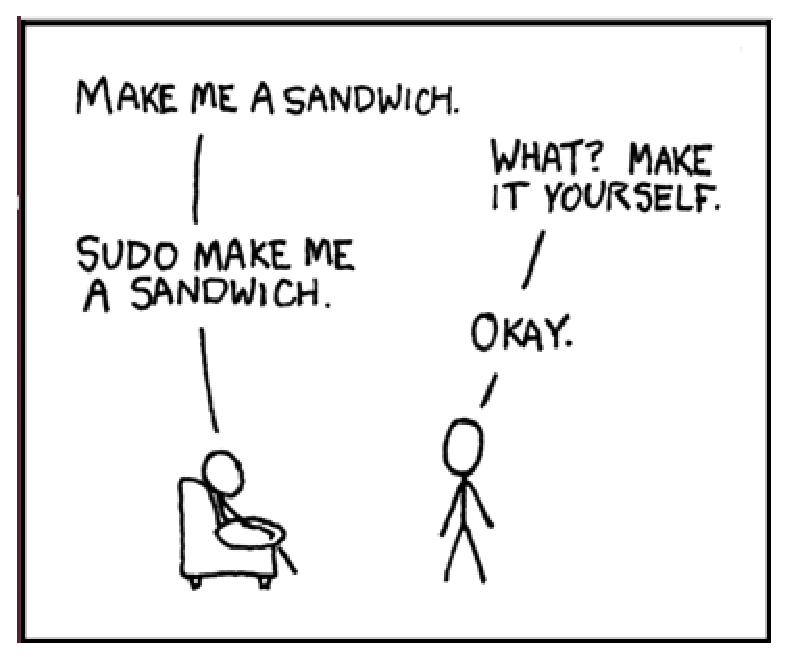
\includegraphics[clip,width=\columnwidth]{tshirt}
% \end{center}
% \caption{NDP Table: Linux vs USAGI\label{ndp_table}}
%\end{figure}

\end{document}
